\documentclass[conference]{IEEEtran}
\IEEEoverridecommandlockouts

\usepackage{cite}
\usepackage{amsmath,amssymb,amsfonts}
\usepackage{algorithmic}
\usepackage{graphicx}
\usepackage{textcomp}
\usepackage{xcolor}
\usepackage{booktabs}
\usepackage{tabularx}
\usepackage{url}
\usepackage{balance}
\usepackage[hidelinks]{hyperref}

\graphicspath{{figures/}}

\def\BibTeX{{\rm B\kern-.05em{\sc i\kern-.025em b}\kern-.08em
    T\kern-.1667em\lower.7ex\hbox{E}\kern-.125emX}}

\begin{document}

\title{Multi-Task Deep Learning Framework for Unified Cattle Health and Behavior Monitoring}

\author{
\IEEEauthorblockN{1\textsuperscript{st} Hasin Ishrak}
\IEEEauthorblockA{\textit{Dept. of Computer Science} \\
\textit{and Engineering} \\
\textit{BRAC University}\\
Dhaka, Bangladesh \\
hasin.ishrak@g.bracu.ac.bd}
\and
\IEEEauthorblockN{2\textsuperscript{nd} Namira Abrar Haque}
\IEEEauthorblockA{\textit{Dept. of Computer Science} \\
\textit{and Engineering} \\
\textit{BRAC University}\\
Dhaka, Bangladesh \\
namira.abrar.haque@g.bracu.ac.bd}
\and
\IEEEauthorblockN{3\textsuperscript{rd} Sanjida Akter Bithi}
\IEEEauthorblockA{\textit{Dept. of Computer Science} \\
\textit{and Engineering} \\
\textit{BRAC University}\\
Dhaka, Bangladesh \\
sanjida.akter.bithi@g.bracu.ac.bd}
\and[\hfill\mbox{}\par\mbox{}\hfill]
\IEEEauthorblockN{4\textsuperscript{th} Shouvik Banik}
\IEEEauthorblockA{\textit{Dept. of Computer Science} \\
\textit{and Engineering} \\
\textit{BRAC University}\\
Dhaka, Bangladesh \\
shouvik.banik@g.bracu.ac.bd}
\and
\IEEEauthorblockN{5\textsuperscript{th} Nusrat Lamya Faruk}
\IEEEauthorblockA{\textit{Dept. of Computer Science} \\
\textit{and Engineering} \\
\textit{BRAC University}\\
Dhaka, Bangladesh \\
nusrat.lamya.faruk@g.bracu.ac.bd}
}

\maketitle

\begin{abstract}
Automated computer vision in precision livestock farming increasingly targets distinct physiological and behavioral traits, including Body Condition Scoring (BCS), behavior recognition, and individual cow re-identification (Re-ID). These tasks demand distinct visual representations, including static body morphology, temporal posture dynamics, and biometric coat pattern appearance. In this paper, we evaluate task-specific cattle-centered visual representations---incorporating target localization, binary foreground masks, and lightweight temporal modeling---across leakage-aware single-task and multi-task settings over a shared ResNet-18 backbone. We evaluate three multi-task paradigms against matched single-task references: (i) monolithic hard parameter sharing (E1), (ii) modular task-private residual bottleneck adapters (E3), and (iii) gradient conflict projection via PCGrad (E4). Across matched evaluation cohorts (7,549 burst-group-disjoint ScienceDB images, 780 temporal behavior sequences from CVB and Kaggle Beef, and 69 held-out cows evaluated against a 36,811-image gallery under SideView Protocol A), cattle-centered representations provide task-dependent benefits, lowering BCS MAE from $0.1929$ to $0.1709$ and lifting Snapshot Re-ID Rank-1 from $38.88\%$ to $62.93\%$ under oracle mask guidance, while benefits across sub-metrics remain non-uniform. Joint hard sharing (E1) induces outcome-level negative transfer across all three tasks. Task-private adapters (E3, $+3.32\%$ parameters) fail to provide general mitigation. During E4 training, direct diagnostics record 44,177 gradient conflict projections across 16,140 super-steps (46.5\%--47.8\% pairwise conflict frequency). PCGrad provides selective mitigation, notably on Behavior where CVB surveillance accuracy improves ($+4.26$ pp over E1) and minority Walking F1 recovers ($0.0408$ to $0.0909$), though dedicated single-task models remain superior on several primary metrics. Our framework establishes an empirical benchmark demonstrating that multi-task livestock monitoring requires balancing shared representations, task-private capacity, and conflict-aware optimization.
\end{abstract}

\begin{IEEEkeywords}
Precision livestock farming, Multi-task learning, Body condition scoring, Cattle behavior recognition, Cattle re-identification, Gradient conflict, Negative transfer.
\end{IEEEkeywords}

\section{Introduction}
Precision livestock farming (PLF) increasingly relies on automated computer vision to track animal welfare, health, and productivity in dairy and beef operations \cite{weary2009understanding, antognoli2025ani1}. Three visual phenotyping tasks are central to modern herd management: (1) \textit{Body Condition Scoring (BCS)}, which evaluates subcutaneous fat reserves to oversee nutritional status and prevent metabolic disorders \cite{edmonson1989bcs, liu2025vets, yao2026jds2}; (2) \textit{Behavior Recognition}, which monitors feeding, drinking, standing, lying, and locomotion dynamics to detect early lameness or health issues \cite{li2024cbvd5, zia2023cvb}; and (3) \textit{Cow Re-Identification (Re-ID)}, which facilitates non-invasive individual traceability across facility camera viewpoints without physical tags \cite{andrew2017cattle, zhang2026beca}.

Existing systems overwhelmingly execute these tasks through separate, isolated deep neural networks \cite{sani2026ab25, guzhva2026s415}. Maintaining independent single-task vision models presents several practical limitations: (1)~\textit{Excessive Parameter Footprint}: Running separate convolutional backbones for condition scoring, video action recognition, and biometric retrieval triples model storage demands (34.7M parameters across three independent ResNet-18 networks), increasing hardware overhead on rural edge nodes; (2)~\textit{Susceptibility to Background Shortcut Exploitation}: Standard uncropped RGB models risk exploiting non-target background visual features---such as pen manure accumulation, chute metalwork, stall fixtures, or static shadows---rather than invariant anatomical landmarks \cite{geirhos2020shortcut, xiao2021background}; and (3)~\textit{Heterogeneous Demands and Negative Transfer}: Although visual features governing identification and condition assessment share low-level visual representations, naive parameter sharing across heterogeneous spatial and temporal objectives risks gradient conflict and negative transfer \cite{crawshaw2020mtl, standley2020tasks}.

\begin{figure}[t]
\centering
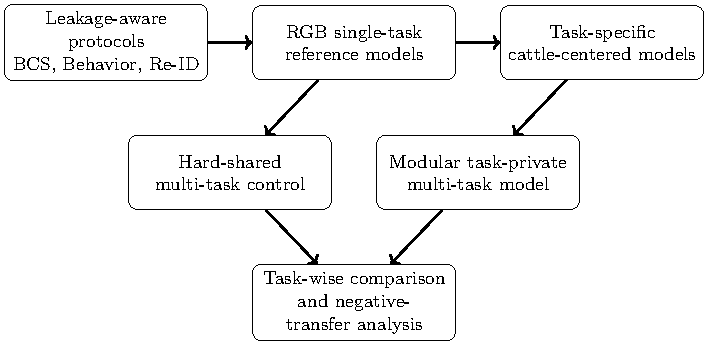
\includegraphics[width=\linewidth]{figures/fig_research_design.pdf}
\caption{Comparative research framework illustrating leakage-aware protocols, single-task baseline references, task-specific cattle-centered representations, and multi-task parameter integration strategies (E1 hard sharing, E3 modular adapters, and E4 PCGrad optimization).}
\label{fig:research_design}
\end{figure}

To address these challenges, we evaluate a multi-task deep learning framework that concurrently assesses body condition scores, 5-class temporal behavior categories, and open-set biometric cow retrieval over a shared 4-channel convolutional backbone (Fig.~\ref{fig:research_design}). We examine whether cattle-centered spatial representations (combining localized cropping and foreground masking) improve individual task outcomes, and evaluate whether modular task-private adapters or gradient surgery can mitigate inter-task negative transfer.

The core contributions of this work are: (1)~\textbf{Evaluation Protocols}: Established verifiable, reliable benchmark protocols for three heterogeneous cattle monitoring domains: a burst-group-disjoint protocol for ScienceDB BCS preventing video frame leakage; a session- and source-disjoint protocol for CVB and Kaggle Beef Behavior; and an identity-disjoint open-set retrieval protocol (SideView Protocol A) evaluating 69 held-out cows against a 36,811-image parlor gallery. (2)~\textbf{Single-Task Baselines on Standard Datasets}: Evaluated standard RGB inputs versus cattle-centered representations across matched test populations, showing that localized cropping and foreground masks reduce BCS MAE from $0.1929$ to $0.1709$ and raise Snapshot Re-ID Rank-1 from $38.88\%$ to $62.93\%$ under oracle masks. (3)~\textbf{Task-Specific Cattle Input Representation}: Formulated a task-tailored representation strategy designing inputs based on task needs: static crops and binary masks for BCS morphology, 8-frame sequences with a lightweight Conv1D temporal network for behavior dynamics, and target-centered crops with oracle masks for re-identification surface patterns, while exploring pose and viewpoint boundaries. (4)~\textbf{Benchmarking for Systematic Multi-Task Sharing}: Conducted controlled multi-task experiments comparing monolithic hard parameter sharing (E1), modular task-private residual adapters (E3), and gradient-projected optimization (E4) against matched single-task baselines on identical test sets, achieving a $65.7\%$ parameter reduction (11.9M vs.\ 34.7M). (5)~\textbf{Direct Gradient Conflict Diagnostics}: Recorded direct empirical evidence of gradient interference on the shared backbone during PCGrad training, capturing 44,177 pairwise conflict projections across 16,140 super-steps ($46.5\%$--$47.8\%$ conflict rate). (6)~\textbf{Calibrated Multi-Task Trade-Offs}: Demonstrated that multi-task learning is not universally advantageous across cattle monitoring tasks due to outcome-level negative transfer, showing that architectural and optimization remedies yield selective, metric-dependent trade-offs rather than uniform improvements.

\section{Related Work}
\textit{1) Body Condition Scoring (BCS):} Body condition scoring assesses an animal's tissue reserves, traditionally conducted via visual inspection on a 5-point scale \cite{edmonson1989bcs, ferguson1994bcs}. Earlier automated studies explored 3D surface imaging and depth sensors to analyze pelvic and tailhead depressions \cite{rodriguez2018bcs}. Recent works transitioned to 2D deep networks: Liu et al. \cite{liu2025vets} applied attention models to rear chute views, whereas Yao et al. \cite{yao2026jds2} investigated side-view camera systems. However, most existing models formulate BCS as standard continuous regression or unordered multiclass classification. Although ordinal methods like CORAL \cite{coral2020} constrain rank cutoffs, our framework implements independent ordinal binary cross-entropy over four cumulative threshold logits, predicting discrete score boundaries directly.

\textit{2) Cattle Behavior Recognition:} Automated cattle behavior monitoring focuses on recognizing fundamental activities such as feeding, standing, lying, and locomotion \cite{weary2009understanding}. Previous approaches relied on heavy 3D convolutions or optical flow, which incur substantial computational cost and suffer under camera shake \cite{feichtenhofer2019slowfast}. Open datasets such as CVB \cite{zia2023cvb} and CBVD \cite{li2024cbvd5} enable efficient combinations of 2D convolutional encoders with 1D temporal networks \cite{bai2018tcn}. However, networks trained on raw unsegmented surveillance feeds risk learning shortcut correlations from static background elements like fences or stalls \cite{geirhos2020shortcut}, even though scene context can occasionally provide informative cues.

\textit{3) Individual Cattle Re-Identification:} Individual cattle re-identification provides non-invasive tracking across agricultural facilities without relying on physical ear tags. Studies by Andrew et al. \cite{andrew2017cattle, andrew2021opencows} showed that natural coat markings and body contours of Holstein cattle serve as reliable biometric patterns. Recent open-set retrieval architectures utilize deep embedding spaces optimized with cross-entropy loss and cosine similarity matching \cite{zhang2026beca}. Nevertheless, environmental shifts between indoor parlors and outdoor pens lead to noticeable retrieval drops when lighting, cattle pose, and camera perspectives change substantially.

\textit{4) Multi-Task Learning and Gradient Balancing:} Multi-task learning seeks to share representational features across related vision problems, reducing computational overhead while enhancing generalization \cite{crawshaw2020mtl}. However, naive parameter sharing regularly results in negative transfer, wherein task competition degrades performance relative to dedicated single-task baselines \cite{standley2020tasks}. Architectural strategies employ modular adapters or specialized routing layers \cite{misra2016crossstitch, liu2019mtan}. Optimization methods address gradient interference: GradNorm dynamically adjusts task loss weights \cite{chen2018gradnorm}, whereas PCGrad projects conflicting gradients onto normal planes whenever directional conflicts arise \cite{yu2020pcgrad}. This study systematically contrasts hard sharing (E1), modular task-private adapters (E3), and gradient projection (E4) across multi-modal livestock monitoring.

\section{Proposed Methodology}

\begin{figure*}[t]
\centering
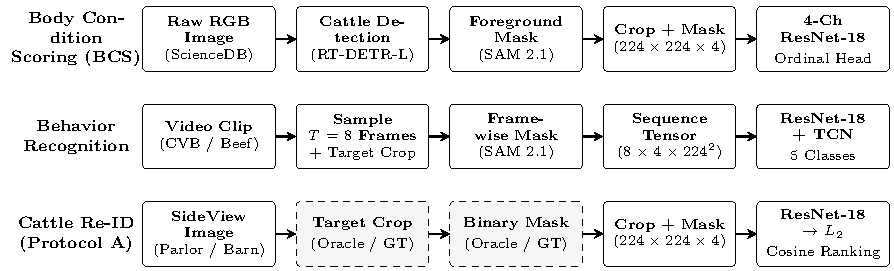
\includegraphics[width=\textwidth]{figures/fig_input_pipeline.pdf}
\caption{Task-specific cattle-centered input representation pipelines across Body Condition Scoring (ScienceDB), Behavior Recognition (CVB / Beef), and Cattle Re-Identification (SideView Protocol A). Target localization, bounding-box cropping, and binary foreground masks generate standardized 4-channel input tensors ($224 \times 224 \times 4$), with Re-ID evaluated under released oracle ground-truth masks.}
\label{fig:input_pipeline}
\end{figure*}

\subsection{Task-Specific Cattle-Centered Perception Pipelines}
Because the three monitoring domains differ in visual and temporal requirements, the cattle-centered models focus on the target cow using task-specific preprocessing rather than an identical automated pipeline (Fig.~\ref{fig:input_pipeline}):
\begin{enumerate}
    \item \textbf{Body Condition Scoring (ScienceDB)}: RT-DETR-L \cite{zhao2024rtdetr} detects cattle using the COCO cattle class with a confidence threshold of 0.25. If multiple cattle are detected, the largest bounding box is selected, and confidence breaks ties. The selected box is expanded by approximately 5\% in each direction, clipped to the image boundary, and used for both the RGB crop and the SAM 2.1 prompt \cite{ravi2024sam2}. SAM 2.1 generates a binary mask in $\{0, 1\}$. Both RGB and mask are resized to $224 \times 224$. RGB channels use ImageNet normalization, while the fourth channel remains an unnormalized binary mask. Perception failures (detector misses or empty masks) are excluded; no artificial replacement input is used.
    \item \textbf{Behavior Recognition (CVB + Beef)}: For CVB video clips, target-tracklet bounding boxes provided by the dataset at each sampled frame prompt SAM 2.1, and the identical box coordinates are applied to RGB and mask crops. For single-cow Kaggle Beef clips, RT-DETR-L provides the animal bounding box when available, followed by a positive center prompt to SAM 2.1; if the detector finds no cow, an image-center prompt is used. A sequence is excluded if any required mask is empty or invalid.
    \item \textbf{Cattle Re-Identification (SideView Protocol A)}: SideView Re-ID experiments utilize the released ground-truth target-cow segmentation masks, operating strictly as an \textit{oracle segmentation-guided experiment}. The non-zero region of the ground-truth mask defines the bounding box, which is expanded by approximately 5\%. The same crop coordinates are applied to both RGB and mask, resizing both to $224 \times 224$. The binary fourth channel is concatenated with ImageNet-normalized RGB; RGB pixels are not multiplied by the mask.
\end{enumerate}

\subsection{Shared Spatial Trunk and Task-Specific Heads}
The shared visual representation is parameterized by a 4-channel ResNet-18 backbone (11,179,648 parameters) \cite{he2016resnet}. The first convolutional layer is expanded from $\mathbb{R}^{64 \times 3 \times 7 \times 7}$ to $\mathbb{R}^{64 \times 4 \times 7 \times 7}$, with the new mask-channel weights initialized to the mean of the three pretrained RGB filters. For an input image, the trunk yields a 512-dimensional spatial feature vector $\mathbf{h} \in \mathbb{R}^{512}$.

\textit{1) BCS Ordinal Regression Head:} ScienceDB BCS targets comprise five ordered discrete classes: 3.25, 3.50, 3.75, 4.00, and 4.25. For a class index $y \in \{0, 1, 2, 3, 4\}$, four independent cumulative threshold targets are defined: $t_k = \mathbb{I}(y > k), k \in \{0, 1, 2, 3\}$. The BCS linear head (2,052 parameters) produces four threshold logits $g_k = \mathbf{w}_k^\top \mathbf{h} + b_k$. The loss is independent ordinal binary cross-entropy:
\begin{equation}\label{eq:bcs_loss}
\begin{aligned}
L_{\mathrm{BCS}} = -\frac{1}{4B}\sum_{i=1}^{B}\sum_{k=0}^{3} \big[ & t_{ik}\log\sigma(g_{ik}) \\
& + (1-t_{ik})\log(1-\sigma(g_{ik})) \big].
\end{aligned}
\end{equation}
During inference, the discrete class index is determined by counting threshold probabilities exceeding 0.5, then mapped back to the physical BCS scale: $\hat{y} = \sum_{k=0}^{3} \mathbb{I}(\sigma(g_k) > 0.5), \widehat{\mathrm{BCS}} = 3.25 + 0.25\hat{y}$.

\textit{2) Temporal Behavior Recognition Head:} For video clips, $T=8$ approximately evenly spaced frames are extracted per sample, producing input tensor $[B, 8, 4, 224, 224]$. The shared 4-channel trunk processes each frame independently, yielding temporal feature sequence $\mathbf{H} \in \mathbb{R}^{B \times 8 \times 512}$. A lightweight residual Conv1D model over these frame features performs sequence modeling: the first block applies a width-three Conv1D projection from 512 to 256 channels, BatchNorm, GELU, dropout (0.2), and a width-one residual projection; the second block maintains 256 channels with BatchNorm, GELU, dropout (0.2), and an identity residual. Temporal adaptive average pooling produces a 256-dimensional feature routed to a 5-class linear classifier (723,973 parameters in head; 11,903,621 total). The head is optimized via categorical cross-entropy $L_{\mathrm{Beh}}$.

\textit{3) Biometric Re-Identification Head:} During representation learning on the 41 parlor training cows, the raw 512-dimensional feature $\mathbf{h}$ is passed to a 41-class linear classifier with bias (21,033 parameters) optimized with categorical cross-entropy loss $L_{\mathrm{ReID}}$. For open-set retrieval evaluation across unseen cows, the retrieval embedding is formed by $L_2$ unit normalization: $\mathbf{z} = \mathbf{h} / \|\mathbf{h}\|_2$. The retrieval embedding remains 512-dimensional. Cosine similarity between normalized query and gallery embeddings ranks candidate identities.

\begin{figure*}[t]
\centering
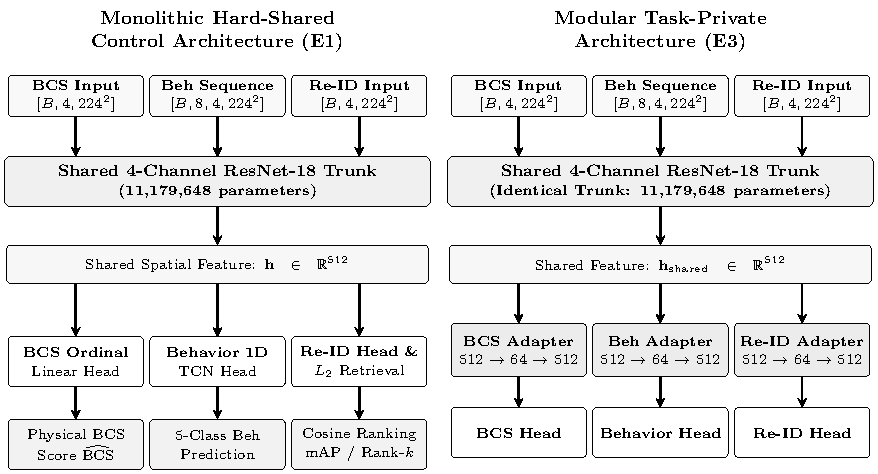
\includegraphics[width=\textwidth]{figures/fig_mtl_architecture.pdf}
\caption{Comparison of multi-task learning architectures. Left: Monolithic hard-shared control (E1) routing a single 512-dim trunk feature to all three heads. Right: Modular task-private architecture (E3) inserting bottleneck residual adapters ($512 \to 128 \to 512$) to decouple task-specific capacity.}
\label{fig:mtl_architecture}
\end{figure*}

\subsection{Multi-Task Architectural Paradigms}
\textit{1) Monolithic Hard-Shared Baseline (E1):} As depicted in Fig.~\ref{fig:mtl_architecture} (left), all three task heads branch directly from the single shared 4-channel ResNet-18 trunk (11,179,648 shared parameters; 93.74\% of total capacity). Total trainable parameters equal 11,926,706. Shared trunk parameters $\boldsymbol{\theta}_{\mathrm{shared}}$ are updated via direct summation: $\mathbf{g}_{\mathrm{shared}} = \mathbf{g}_{\mathrm{BCS}} + \mathbf{g}_{\mathrm{Beh}} + \mathbf{g}_{\mathrm{ReID}}$.

\textit{2) Modular Task-Private Residual Adapters (E3):} To evaluate whether task-private capacity mitigates negative transfer, E3 inserts an independent residual bottleneck adapter ($512 \to 128 \to 512$) between the shared feature $\mathbf{h}_{\mathrm{shared}}$ and each task head (Fig.~\ref{fig:mtl_architecture}, right). Each adapter contains a linear down-projection $\mathbf{W}_{\mathrm{down}} \in \mathbb{R}^{128 \times 512}$, Layer Normalization, GELU activation, dropout ($p=0.1$), and a linear up-projection $\mathbf{W}_{\mathrm{up}} \in \mathbb{R}^{512 \times 128}$. The adapter output $\Delta\mathbf{h}_t$ is added residually: $\mathbf{h}_t = \mathbf{h}_{\mathrm{shared}} + \Delta\mathbf{h}_t$. In Behavior, the adapter operates frame-wise across all 8 frame embeddings before temporal convolution. The up-projection is initialized to zero ($\mathbf{W}_{\mathrm{up}} = \mathbf{0}, \mathbf{b}_{\mathrm{up}} = \mathbf{0}$), ensuring identity initialization ($\Delta\mathbf{h}_t = \mathbf{0}$) at step zero. Each adapter adds 131,968 parameters (395,904 total; $+3.32\%$ capacity), yielding 12,322,610 trainable parameters.

\begin{figure*}[t]
\centering
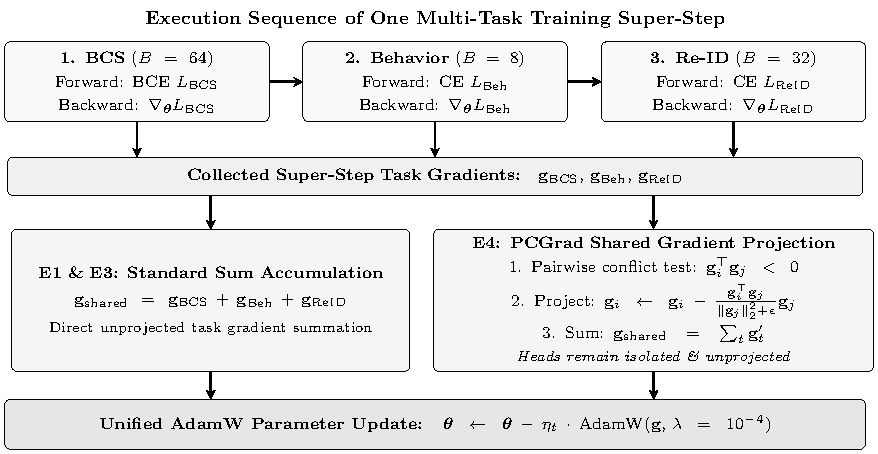
\includegraphics[width=\textwidth]{figures/fig_superstep_routing.pdf}
\caption{Execution sequence and gradient routing of one multi-task training super-step. Sequential micro-batch gradients are accumulated; in E4 (PCGrad), conflicting shared trunk gradients ($\mathbf{g}_i^\top \mathbf{g}_j < 0$) are projected onto normal planes before the unified AdamW update.}
\label{fig:superstep_routing}
\end{figure*}

\textit{3) Gradient-Projected Optimization via PCGrad (E4):} E4 evaluates optimization-level conflict resolution while preserving the exact parameterization of E1 (11,926,706 trainable parameters; 0 adapters, 0 gates). When a pair of task gradients on the shared trunk conflicts ($\mathbf{g}_i^\top \mathbf{g}_j < 0$), $\mathbf{g}_i$ is projected onto the normal plane of $\mathbf{g}_j$ \cite{yu2020pcgrad}:
\begin{equation}
\mathbf{g}_i \leftarrow \mathbf{g}_i - \frac{\mathbf{g}_i^\top \mathbf{g}_j}{\|\mathbf{g}_j\|_2^2 + \epsilon} \mathbf{g}_j.
\end{equation}
Pairwise projection order is deterministically shuffled at each step. Modified shared gradients are summed ($\mathbf{g}_{\mathrm{shared}} = \sum_t \mathbf{g}'_t$). Task-head gradients remain unprojected.

\subsection{Super-Step Multi-Task Training Protocol}
Because commercial cattle datasets do not share overlapping annotations across condition, behavior, and identity, joint training employs interleaved mini-batch super-steps (Fig.~\ref{fig:superstep_routing}): (1) BCS forward/backward ($B_{\mathrm{BCS}} = 64$); (2) Behavior forward/backward ($B_{\mathrm{Beh}} = 8$ video sequences / 64 frames); (3) Re-ID forward/backward ($B_{\mathrm{ReID}} = 32$). Task loss weights are equal ($w_{\mathrm{BCS}} = w_{\mathrm{Beh}} = w_{\mathrm{ReID}} = 1.0$).

Training executes for 30 epochs with 538 super-steps per epoch (16,140 total super-steps), determined by the complete ScienceDB training population ($\lceil 34{,}369 / 64 \rceil = 538$). Optimization uses AdamW (initial learning rate $10^{-4}$, cosine decay to $10^{-6}$, weight decay $10^{-4}$, seed 2026). Checkpoint selection is strictly determined by minimizing the composite validation objective: $L_{\mathrm{MTL,val}} = \frac{1}{3}( L_{\mathrm{BCS,val}} + L_{\mathrm{Beh,val}} + L_{\mathrm{ReID,val}} )$.

\section{Experimental Setup and Benchmark Datasets}

\subsection{Benchmark Datasets and Leakage Prevention}
Rigorous validation in livestock vision requires preventing identity and background leakage across splits:
\textit{1) BCS (ScienceDB):} ScienceDB contains 53,566 RGB images across five discrete scores (3.25 to 4.25) \cite{sciencedb2024bcs}. Verified biological cow IDs are not available. To prevent near-identical video frame leakage, we enforce a repaired burst-group-disjoint protocol across 5,653 canonical burst groups: train (37,045 images; 3,958 bursts), validation (8,481 images; 850 bursts), and test (8,040 images; 845 bursts). The matched perception-successful test evaluation cohort covers 7,549 images ($93.89\%$ coverage; 489 detection misses and 2 empty masks excluded).

\textit{2) Behavior Recognition (CVB + Beef):} Combines CVB open-pasture surveillance video (66 source videos) \cite{zia2023cvb} and Kaggle Beef feedlot clips (201 recording sessions) \cite{lucyfirst2023beef}, comprising 267 protected groups and 5,274 samples. Canonical split: train (3,785), validation (680), test (809). Walking occurs exclusively in CVB. Matched test comparison evaluates 780 retained sequences (422 CVB, 358 Beef; 29 stanchion occlusions excluded). Evaluation is source/session-group-disjoint, not cow-disjoint.

\textit{3) Cattle Re-ID (SideViewCows2026):} Contains 80,260 images and 80,260 masks across 110 cows \cite{moeller2026sideview}. Under Protocol A, 41 cows are used for representation learning (12,753 train, 2,683 val in parlor), while 69 held-out cows form the evaluation set. A fixed parlor gallery of 36,811 images is evaluated against 25,260 barn queries and 607 snapshot queries (covering 63 cows). Evaluations use released ground-truth masks (oracle benchmark).

\subsection{Implementation Details}
Models were trained using PyTorch on NVIDIA L40S GPUs. All single-task and multi-task models are evaluated from single validation-selected checkpoints (point estimates). Held-out test sets remained fully isolated from training, hyperparameter tuning, and threshold selection.

\section{Experimental Results and Analysis}

\subsection{Single-Task Baselines vs Cattle-Centered Perception}
Table~\ref{tab:singletask_results} reports single-task performance comparing raw RGB models against cattle-centered 4-channel configurations on matched evaluation cohorts.

\begin{table}[htbp]
\caption{Single-Task Baselines (Runs 1--3) vs Cattle-Centered Perception (Runs 4--6) on Matched Evaluation Cohorts}
\label{tab:singletask_results}
\centering
\footnotesize
\setlength{\tabcolsep}{3.5pt}
\begin{tabularx}{\linewidth}{l X c c}
\toprule
\textbf{Task} & \textbf{Evaluation Metric} & \textbf{RGB} & \textbf{Cattle-Cent.} \\
\midrule
\textbf{BCS} & Real MAE $\downarrow$ & 0.1929 & \textbf{0.1709} \\
& Exact Acc@0 (\%) $\uparrow$ & 40.84 & \textbf{43.57} \\
& Tol. Acc@1 (\%) $\uparrow$ & 84.95 & \textbf{89.40} \\
& Macro-F1 $\uparrow$ & \textbf{0.4074} & 0.4039 \\
\midrule
\textbf{Behavior} & Overall Acc (\%) $\uparrow$ & \textbf{88.46} & 87.44 \\
& Balanced Acc (\%) $\uparrow$ & 71.30 & \textbf{74.43} \\
& Macro-F1 $\uparrow$ & 0.7378 & \textbf{0.7397} \\
& CVB Surveillance Acc (\%) $\uparrow$ & \textbf{84.12} & 80.09 \\
\midrule
\textbf{Re-ID} & Barn$\to$Parlor R-1 (\%) $\uparrow$ & 58.64 & \textbf{63.90} \\
(Proto A) & Barn$\to$Parlor mAP (\%) $\uparrow$ & 38.32 & \textbf{40.68} \\
& Snap$\to$Parlor R-1 (\%) $\uparrow$ & 38.88 & \textbf{62.93} \\
& Snap$\to$Parlor mAP (\%) $\uparrow$ & 27.05 & \textbf{40.42} \\
\bottomrule
\end{tabularx}
\end{table}

The single-task evaluations demonstrate that benefits are task-dependent and non-uniform across metrics:

\textit{1) BCS Prediction:} In the BCS single-task evaluation, cropping and binary masks achieved superior performance compared to the standard RGB baseline. MAE decreased from 0.1929 to 0.1709 BCS units, and tolerance accuracy within $\pm$0.25 (Acc@1) rose from 84.95\% to 89.40\% (+4.45 pp), though exact accuracy was 43.57\%. Balanced accuracy and Macro-F1 dropped slightly (from 40.23\% to 39.70\% and from 0.4074 to 0.4039), showing that foreground isolation concentrated prediction errors around true score thresholds without altering discrete class-balanced metrics.

\textit{2) Behavior Recognition:} For behavior monitoring, cropped cattle images, foreground masks, and a 1D temporal network outperformed single-frame RGB models across several metrics. Balanced accuracy rose from 71.30\% to 74.43\% (+3.13 pp), test loss decreased from 0.5505 to 0.4430, and Walking F1 improved from 0.2174 to 0.2456. However, overall accuracy dropped slightly from 88.46\% to 87.44\%, with the approach proving more effective on feedlot camera views and somewhat less effective on CVB barn surveillance (80.09\% vs 84.12\%).

\textit{3) Cattle Re-ID:} Re-identification models were evaluated across 69 unseen cattle using SideView Protocol A. Target-centered crops derived from oracle ground-truth masks boosted first-match accuracy across both query scenarios: Barn-to-Parlor Rank-1 increased from 58.64\% to 63.90\% (mAP from 38.32\% to 40.68\%), while Snapshot-to-Parlor Rank-1 improved from 38.88\% to 62.93\% (+24.05 pp; mAP from 27.05\% to 40.42\%), proving particularly advantageous under extreme pose, viewpoint, and lighting variations.

Because localization, cropping, binary masks, and temporal convolutions were applied jointly, observed performance gains reflect complete pipeline configurations rather than segmentation alone.

\begin{figure}[t]
\centering
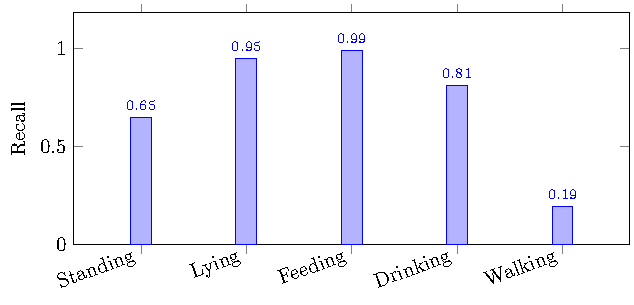
\includegraphics[width=\linewidth]{figures/fig_behavior_recall.pdf}
\caption{Single-task behavior recall across 5 action categories on held-out test data. Sedentary postures (feeding, lying) achieve high recall, while walking represents an underrepresented minority class.}
\label{fig:behavior_recall}
\end{figure}

\subsection{Multi-Task Learning Performance and Negative Transfer}
Table~\ref{tab:mtl_results} presents the comparative evaluation across the three multi-task models against the single-task cattle-centered reference (E0).

\begin{table*}[t]
\caption{Held-Out Evaluation Across Single-Task Reference (E0) and Multi-Task Architectures (E1 Hard-Shared, E3 Modular, E4 PCGrad)}
\label{tab:mtl_results}
\centering
\small
\begin{tabularx}{\textwidth}{l X c c c c}
\toprule
\textbf{Task / Domain} & \textbf{Evaluation Metric} & \textbf{Single-Task (E0)} & \textbf{Hard-Shared (E1)} & \textbf{Modular E3} & \textbf{PCGrad (E4)} \\
\midrule
\textbf{BCS Evaluation} & Real MAE $\downarrow$ & \textbf{0.1709} & 0.1788 & 0.1916 & 0.1828 \\
(ScienceDB Test) & Tolerance Acc@1 (\%) $\uparrow$ & \textbf{89.40} & 88.44 & 86.32 & 87.84 \\
& Exact Acc@0 (\%) $\uparrow$ & \textbf{43.57} & 41.10 & 38.47 & 40.23 \\
& Macro-F1 $\uparrow$ & \textbf{0.4039} & 0.3605 & 0.3291 & 0.3516 \\
\midrule
\textbf{Behavior Evaluation} & Overall Accuracy (\%) $\uparrow$ & \textbf{87.44} & 85.00 & 85.77 & 86.92 \\
(CVB + Beef) & Balanced Accuracy (\%) $\uparrow$ & \textbf{74.43} & 67.30 & 66.70 & 69.15 \\
& Macro-F1 $\uparrow$ & \textbf{0.7397} & 0.6866 & 0.6755 & 0.7114 \\
& CVB Surveillance Acc (\%) $\uparrow$ & 80.09 & 76.78 & 80.33 & \textbf{81.04} \\
& CVB Surveillance F1 $\uparrow$ & \textbf{0.6188} & 0.5402 & 0.6026 & 0.6141 \\
& Minority Walking F1 $\uparrow$ & \textbf{0.2456} & 0.0408 & 0.0000 & 0.0909 \\
\midrule
\textbf{Re-ID Protocol A} & Query Barn $\to$ Parlor Rank-1 (\%) $\uparrow$ & \textbf{63.90} & 57.38 & 49.08 & 54.97 \\
(Held-Out Cows) & Query Barn $\to$ Parlor mAP (\%) $\uparrow$ & \textbf{40.68} & 30.37 & 28.04 & 30.23 \\
& Query Snap $\to$ Parlor Rank-1 (\%) $\uparrow$ & \textbf{62.93} & 57.17 & 53.71 & 57.00 \\
& Query Snap $\to$ Parlor mAP (\%) $\uparrow$ & \textbf{40.42} & 33.69 & 28.78 & 33.87 \\
\midrule
\textbf{Efficiency} & Total Trainable Parameters & 34,706,006 ($3\times$) & \textbf{11,926,706} & 12,322,610 & \textbf{11,926,706} \\
& Relative Parameter Footprint & $100\%$ & \textbf{34.3\%} & 35.5\% & \textbf{34.3\%} \\
\bottomrule
\end{tabularx}
\end{table*}

\textit{1) Negative Transfer in Hard Sharing (E1):} Hard parameter sharing (E1) resulted in outcome-level negative transfer across all three tasks compared to matched single-task baselines: BCS MAE degraded from 0.1709 to 0.1788; Behavior balanced accuracy fell from 74.43\% to 67.30\% (Walking F1 dropping from 0.2456 to 0.0408); and Re-ID Barn Rank-1 declined from 63.90\% to 57.38\% (mAP dropping from 40.68\% to 30.37\%). Restricting diverse cattle vision tasks to a single shared ResNet-18 spatial backbone directly caused this cross-task interference.

\textit{2) Modular Bottleneck Adapters (E3):} Incorporating task-private residual bottleneck adapters (E3) had minimal impact on mitigating negative transfer. While E3 improved Behavior test loss (0.4193) and CVB surveillance accuracy (80.33\%) over E1, BCS MAE worsened to 0.1916, Re-ID Barn Rank-1 dropped to 49.08\% (mAP 28.04\%), and Walking F1 collapsed to 0.0000 on the matched held-out test set. Moreover, because E3 added 395,904 trainable parameters (+3.32\% capacity over E1), performance variations cannot be attributed solely to architectural routing.

\textit{3) Selective Mitigation via PCGrad (E4):} Optimization control with PCGrad (E4) preserved exact parameter parity with E1 (11,926,706 parameters). Projecting conflicting gradients provided selective mitigation: Behavior overall accuracy reached 86.92\% ($+1.92$ pp vs E1), balanced accuracy rose to 69.15\% ($+1.85$ pp), Macro-F1 reached 0.7114 ($+0.0248$), CVB surveillance accuracy reached 81.04\% ($+4.26$ pp), and Walking F1 recovered to 0.0909 (vs.\ 0.0408 in E1), while recovering key BCS and Re-ID metrics relative to E3. Nonetheless, E4 did not eliminate negative transfer, with dedicated single-task models retaining superiority on several primary metrics (BCS MAE 0.1709 vs 0.1828; Behavior balanced accuracy 74.43\% vs 69.15\%; Walking F1 0.2456 vs 0.0909; Barn Rank-1 63.90\% vs 54.97\%).

\subsection{Shared-Backbone Gradient Conflict Diagnostics}
Direct optimization diagnostics recorded \textbf{44,177 gradient conflict projections} across 16,140 super-steps (averaging $2.737$ projections per super-step) during E4 training on the shared 4-channel ResNet-18 backbone. Opposing gradient directions occurred regularly across task pairings with conflict frequencies between 46.5\% and 47.8\% (BCS vs Behavior: 47.8\%; BCS vs Re-ID: 46.5\%; Behavior vs Re-ID: 47.4\%). This demonstrates regular gradient conflict during multi-task cattle training. However, these diagnostics were captured specifically during E4 execution; they do not prove that gradient conflict was the sole causal driver of E1 degradation, nor that E1 exhibited identical conflict statistics.

\section{Discussion, Uncertainty, and Claim Boundaries}
\textit{1) Cross-Task Representation Trade-Offs:} The findings demonstrate that cattle-centered visual representations provide clear utility for individual tasks, but benefits depend on task-specific requirements: body morphology for BCS, temporal movement for behavior, and unique coat markings for Re-ID. Forcing these disparate tasks to share a ResNet-18 backbone induces outcome-level negative transfer. Neither task-private adapters (E3) nor gradient projection (E4) universally eliminated this conflict. Dedicated single-task models remained superior across primary task criteria. While multi-task consolidation reduces parameter footprint by $65.7\%$ (11.9M vs 34.7M parameters), practical deployment represents an engineering compromise against single-task accuracy.

\textit{2) Statistical Boundaries and Point Estimates:} All evaluated models reflect single validation-selected checkpoints (point comparisons). Due to computational constraints, repeated-seed training distributions, confidence intervals, and hypothesis tests were not conducted. Reported differences represent descriptive point comparisons and are not framed as statistically significant. Although the matched evaluation design guarantees strict internal comparability across identical cohorts (7,549 ScienceDB images, 780 Behavior sequences, 69 held-out Re-ID cows), it does not quantify seed-level variance.

\textit{3) Methodological Limitations:} To preserve scientific claim boundaries, key limitations must be stated explicitly: (i) ScienceDB does not verify biological cow IDs; the burst-group-disjoint protocol prevents frame leakage from passage sequences but cannot guarantee biological cow-disjoint evaluation. (ii) Behavior data are partitioned by video sessions rather than cow identities, with minority Walking appearing solely in CVB surveillance (26 test sequences), creating an inherent camera-activity association. (iii) Automated perception retained 93.89\% of ScienceDB images (7,549 / 8,040) and 96.42\% of Behavior sequences (780 / 809); instances with perception failure remain outside the evaluated distribution. (iv) Re-ID models utilized released ground-truth masks; this oracle benchmark does not evaluate automated upstream segmentation. (v) localization, cropping, binary masks, and temporal convolutions were evaluated jointly, precluding isolated component attribution. (vi) E3 introduced 395,904 additional parameters (+3.32\%), confounding routing with capacity. (vii) External stress tests on uncalibrated datasets remain unexecuted roadmap items. (viii) High pose keypoint missingness on recumbent cows (72.92\% failure on lying cattle) and source shortcut risks prevented pose/viewpoint integration in downstream models.

\section{Conclusion and Future Work}
This study developed and evaluated an empirical framework for multi-task deep learning in precision cattle monitoring across BCS, behavior recognition, and individual re-identification under controlled protocols. Cattle-centered representations improved BCS error tolerance and enhanced re-identification under substantial camera shifts, though improvements were task-dependent and non-uniform across metrics. Hard parameter sharing induced outcome-level negative transfer across all three tasks. Task-private adapters failed to resolve this degradation, while PCGrad delivered selective mitigation---notably improving CVB surveillance accuracy and minority walking classification---under parameter parity with hard sharing. Dedicated single-task models remained superior on several primary metrics, demonstrating that multi-task livestock monitoring requires balancing shared efficiency, task-private capacity, and conflict-aware optimization.

Future research will explore: (1) repeated seed training to estimate confidence intervals and variance bounds; (2) end-to-end automated segmentation replacing oracle masks in re-identification; (3) cross-farm generalization on independent external herds; (4) longitudinal biometric evaluation across lactation stages and coat growth; (5) factorial ablations for isolated perception components; (6) robust animal pose estimation for recumbent and rear postures; and (7) partial parameter sharing with adaptive loss weighting (e.g., GradNorm \cite{chen2018gradnorm}) to resolve cross-task gradient conflict.

\section*{Acknowledgment}
The authors thank the Department of Computer Science and Engineering, BRAC University, for computational facilities, Dr. Md. Khalilur Rahman for thesis supervision, and Mehedi Hasan Emo and Mollah MD Saif for guidance throughout this research.

\balance
\bibliographystyle{IEEEtran}
\bibliography{references}

\end{document}
